% Generated by to_latex.py from perspective.rsm. Do not edit by hand.
\documentclass[utf8]{FrontiersinHarvard}
\usepackage{url,hyperref,lineno,microtype,subcaption}
\usepackage[onehalfspacing]{setspace}

\linenumbers

\def\keyFont{\fontsize{8}{11}\helveticabold }
\def\firstAuthorLast{Torres}
\def\Authors{Leo Torres\,$^{*}$}
\def\Address{Independent researcher, Leipzig, Germany}
\def\corrAuthor{Leo Torres}
\def\corrEmail{leo@leotrs.com}

\begin{document}
\onecolumn
\firstpage{1}

\title[Three readings of group interactions]{Group interactions in the data, in the best model, or in the system}

\author[\firstAuthorLast ]{\Authors}
\address{}
\correspondance{}

\extraAuth{}

\maketitle

\begin{abstract}

\section{}
Studies of higher-order networks often justify representing the data as a hypergraph by the claim that the system under study has group interactions. We distinguish three readings of this claim: about how the data were recorded, about which model predicts them best, and about how the system works. Each reading needs its own evidence. Model selection on recorded data, which Rommens et al. propose in this Research Topic as a test of such claims, can provide evidence for the second only. We run a synthetic benchmark of the kind that they propose. We simulate people who meet in gatherings and adopt a behavior via a pairwise mechanism, a group mechanism, or a mix of the two. The gatherings are recorded in two different modalities: a meeting log and proximity sensors. Like Rommens et al., we compare models by message length: the number of bits needed to encode the recorded structure, the rule of the dynamics, and the part of the data held out from fitting (a second spreading process) that the model leaves unexplained. In our simulation, whether the hypergraph model has a shorter message length than the graph models depends on how the contacts were recorded and not on the mechanism of spreading. In addition, when adoption depends on groups, wholly or in part, the models fitted to the meeting log give wrong predictions of how a person's chance of adoption changes when the person meets adopters together rather than one at a time. Adding a separate rate for two or more adopters corrects these predictions on the meeting log, but on the sensor record it reports a group effect where there is none, and model selection prefers it. We recommend that authors say which of the three readings of the claim they intend, report separately the bits for encoding the recorded structure and the bits for the rule and for the part of the held-out data that the model leaves unexplained, and test or state the causal assumptions behind any claim about the system.

\tiny
\keyFont{ \section{Keywords:} higher-order networks, hypergraphs, group interactions, model selection, causal inference, interventions}
\end{abstract}

\noindent Number of words in the main text: 2,999. Number of figures and tables: 2.

\section{Introduction}\label{sec-intro}

For much of the history of network science, representing data as a graph required no justification, since it was the unifying and defining practice in the field. The field now has hypergraphs, simplicial complexes, multilayer and temporal networks, and combinations thereof, each with its own models and methods. With alternatives available, ``we built a graph from these data'' no longer suffices, and authors must justify their choice of representation.

When is such a justification valid? For hypergraphs, a common one is the claim that the system under study has group interactions. We distinguish three readings of this claim, each with its own evidence: about how the data were recorded, which model predicts them best, and how the system works. Both sides of the current debate point to model selection to decide between graph and hypergraph models \citep{peixoto2026,arenas2026}. We argue that model selection on recorded data can provide evidence for the second reading only.

We support the argument with a simulated benchmark of the kind that \citet{rommens2026} propose in this Research Topic. They propose to test claims of group interactions by model selection: fit graph and hypergraph models to the same data, and prefer the model that describes three parts together in fewer bits: the recorded structure, the rule of the dynamics, and the data that the model leaves unexplained. In our simulation, the verdict of model selection changes with how the contacts were recorded and not with the mechanism of spreading. When adoption depends on groups, models fitted to a complete record of the contacts underestimate how much meeting adopters together, rather than one at a time, raises the chance of adopting. A model with a separate rate for two or more adopters corrects this, but when the contacts are recorded by proximity sensors that miss some of them, it reports a group effect in a world without one, and model selection prefers it.

\section{Three readings of the claim}\label{sec-argument}

The first reading concerns data collection: observations are recorded as groups, as with meetings, coauthored papers, or emails sent to several recipients. The second concerns prediction: a higher-order model reproduces some feature of the system, such as the spread of a rumor or the coexistence of species, that a pairwise model does not, as measured by statistical fit or, in some studies, by qualitative agreement alone. The third concerns causation in the system itself: the response of one component depends jointly on several others, in a way that does not decompose into pairwise effects \citep{perezreche2026}. The three readings correspond roughly to the three tasks into which data science is commonly divided, description, prediction, and causal inference \citep{hernan2019}, each with its own standard of evidence.

None of the three readings follows from the one before it. Data recorded as groups record how observations were made, not how components influence one another: a meeting of five people may consist entirely of conversations between two. A better fit by a higher-order model than by the graph models compared with it is evidence of a regularity that those models miss, but only relative to them \citep{sober2004} and only in the data as recorded. Neither is evidence for the third reading. In the causal framework generally accepted in data science, such a claim is established by intervention: changing which components are present together and observing the response \citep[p.~417]{pearl2009causality}. Researchers in other fields, notably evolutionary biology, establish causes without experiments, through observation, comparison, and the testing of competing historical explanations \citep{mayr2000}. Here we follow Pearl. With data recorded without changing the system, the effect of an intervention can be computed only from a causal model built from knowledge other than the data, and some of its assumptions cannot be confirmed from the data \citep{pearl2009overview,manski1991,shalizi2011}.

Read as description, the claim is the easiest to justify: by how the data were collected rather than by any analysis of them. The standard for a description is one of measurement: the recorded groups must be the groups that the study is about. A description that meets this standard needs no further support, but it is no evidence for any claim beyond the data as recorded, since the recorded groups are ``co-occurrences rather than demonstrated interactions'' \citep{perezreche2026}.

Read as prediction, the claim is justified by comparing how well models account for data that were not used to fit them, measured by held-out likelihood or estimated by fit penalized for complexity. A higher-order model that wins is the better choice for predicting new data from the same system, whether or not its structure matches how the system works \citep{shmueli2010}. This holds as long as the new data are drawn from the same distribution as the old \citep{breiman2001,sober2002}, which in practice includes being collected with the same instrument. The win has two limits. First, it holds only against the models that were compared. For example, a graph model in which the rate of adoption is nonlinear in the number of adopting neighbors already contains interactions among more than two people \citep{bick2023,peixoto2026}, and adding it to the comparison may change the winner. Second, it holds only while the system runs as it did when the data were collected. Predicting what would happen if the system were changed, for instance if a person met two adopters together rather than one at a time, is a causal question, outside the comparison \citep{hernan2019}.

Read as causation, the claim concerns what would happen if the system were changed. From recorded data, a fitted model answers such a question correctly only under several assumptions, two of which cannot be confirmed from the data: \phantomsection\label{asm-untestable}that the recorded contacts are the routes of spreading, and that who meets whom does not depend on adoption or its causes \citep{pearl2009overview,shalizi2011}. A third is given in Section~\ref{sec-recommendations}.

For the second reading, model selection is certainly the right tool currently at our disposal, and for data recorded without changing the system it is the only tool available. We argue for adding to it: test the causal reading by changing the system when possible and ethical, and otherwise state the causal assumptions on which every causal reading of recorded data rests \citep{pearl2009overview}. Stating them is one way to express in causal terms what \citet{perezreche2026} calls reducibility: whether a higher-order model can be replaced by a lower-order one.

In Section~\ref{sec-study}, we test the argument in a benchmark of the kind that \citet{rommens2026} propose, in which the mechanism is known, and examine its results under each of the three readings.

\section{A simulated benchmark}\label{sec-study}

\subsection{Setup}\label{sec-setup}

\textbf{Event and worlds.} Two hundred people attend a three-day event and meet in gatherings of two to six people that last 15 minutes on average. Each person is in at most one gathering at a time and meets six different people a day on average. Each spreading process starts with 24 people who have adopted a behavior, and adoption is permanent. Spreading is built in three ways, which we call worlds (Figure~\ref{fig-design}A). In the pairwise world, each adopter in a person's gathering converts that person at a constant rate. In the group world, a person adopts at a constant rate while at least two adopters are present, and never with only one. The mixed world has both mechanisms at half strength. In every world, about half of the people adopt.

\textbf{Records.} A run simulates the gatherings and two independent spreading processes of the same world over them. Each run is recorded in two ways, and we call each recording a record (Figure~\ref{fig-design}B). A meeting log lists every gathering with its members, start and end. Proximity sensors sample every 20 seconds and detect each pair in a gathering with probability one half, close to the share of interaction time, about half, that RFID badges detected in a field test against video recordings \citep{elmer2019}. At each sample, the recorded groups are the connected components of the graph of detected pairs. In both records, each person is in at most one recorded group at a time, and the adoption times are included.

\textbf{Models and scores.} Three models give each person who has not adopted a rate of adoption that depends on the contacts recorded at that moment, plus a constant background rate (Figure~\ref{fig-design}C): a linear graph model, in which the rate is linear in the number of adopters in contact (in the same gathering in the meeting log, or detected as a pair in the sensor record); a nonlinear graph model, in which that number is raised to a fitted power; and a hypergraph model, in which the number of adopters in each of the person's recorded groups is raised to a fitted power and the results are summed. Each model is fitted by maximum likelihood to the first spreading process of a run and scored on the second. We use two scores (Figure~\ref{fig-design}D). The message length proposed by \citep{rommens2026} is the sum of three parts: the bits for writing down who met whom in the record (the structure), the bits for writing down the fitted rule, and the misfit, which is minus the base-2 logarithm of the likelihood of the adoption times in the held-out process. The held-out misfit is the last of these alone.

\textbf{Settings.} We changed each of six hyperparameters separately from its main value, for 14 settings in all, each with 20 runs of each world (Figure~\ref{fig-design}E). Supplementary File S1 gives the full specification of the study.

\begin{figure}[h!]
\begin{center}
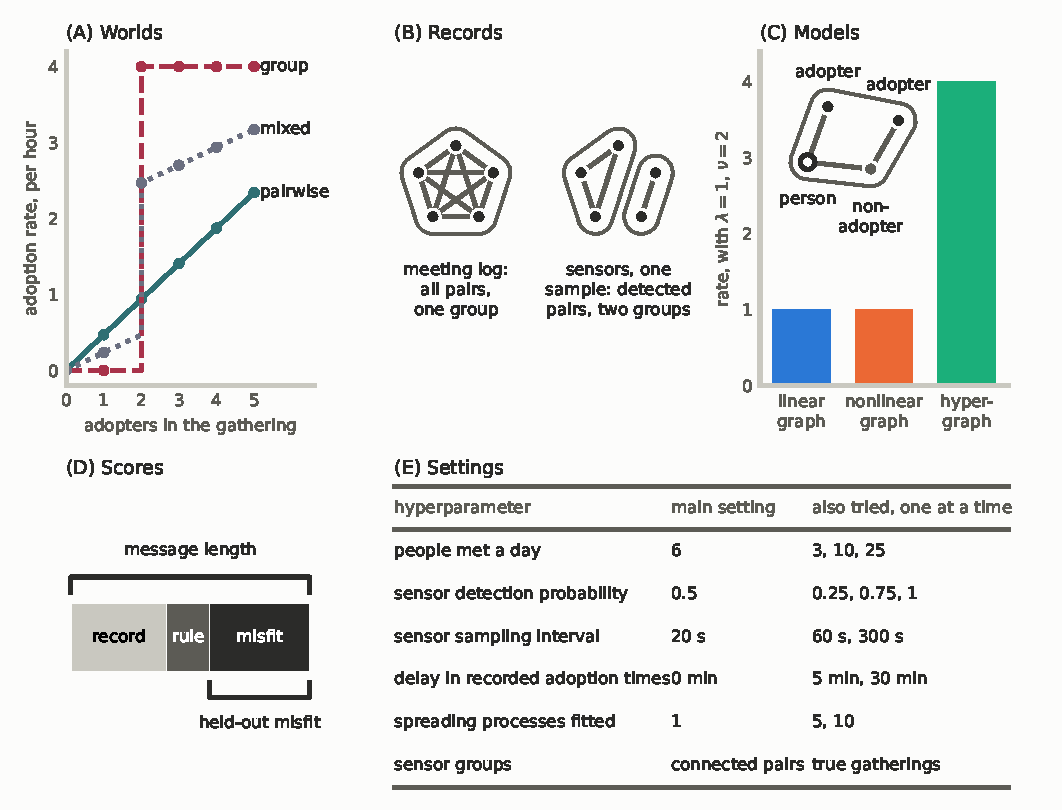
\includegraphics[width=\textwidth]{figure1.pdf}
\end{center}
\caption{Design of the simulated study. (A) Adoption rate in each world. (B) One gathering as recorded by the meeting log and by the sensors at one sample. (C) Rate given by each model to a person whose sensor group holds two adopters, only one of them detected with the person. (D) Parts of the two scores. (E) Hyperparameters: the main setting and the values tried one at a time.}\label{fig-design}
\end{figure}

\subsection{Results}\label{sec-results}

We assess the results under each of the three readings, which follow the division of data science into description, prediction and causal inference (Section~\ref{sec-argument}).

\begin{figure}[h!]
\begin{center}
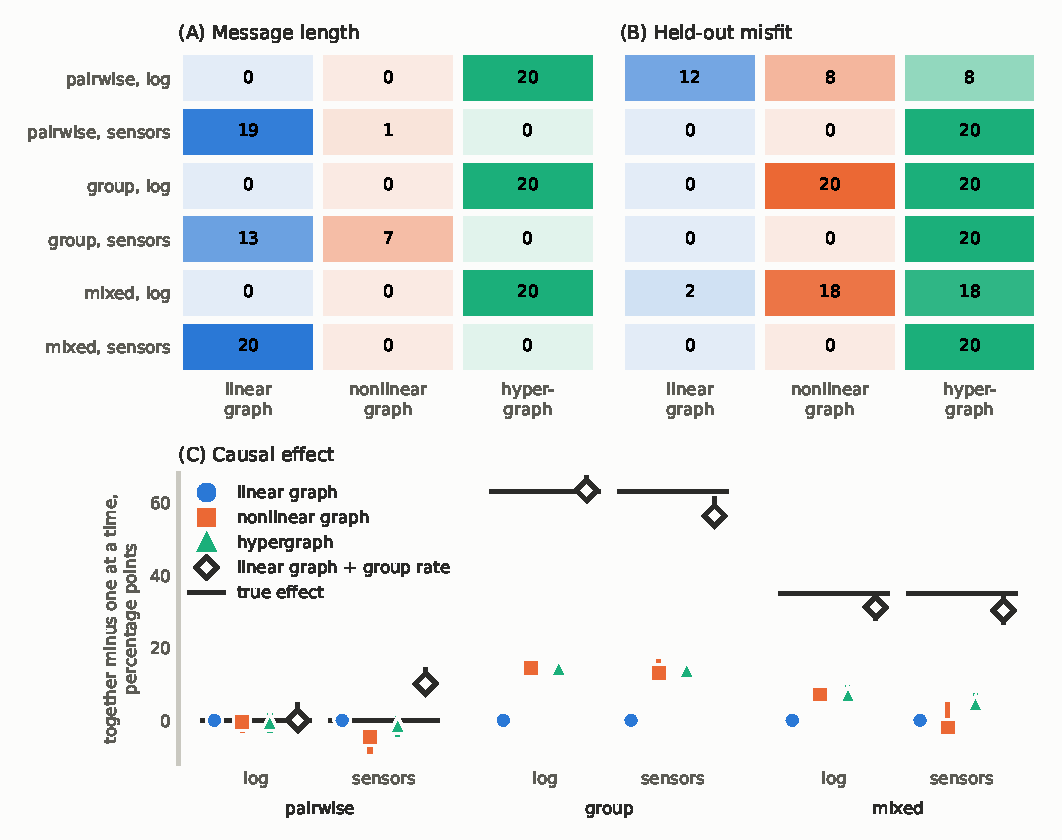
\includegraphics[width=\textwidth]{figure2.pdf}
\end{center}
\caption{Results in the main setting. (A, B) Runs won by each model, out of 20. Models whose scores are equal up to numerical error tie, and a tied run counts for each model in the tie. (C) True effect (bars) and median predicted effect (markers, with interquartile range) of meeting two adopters together rather than one at a time. Hollow diamonds: the linear graph model with an added group rate, which takes no part in the comparisons in A and B.}\label{fig-wins}
\end{figure}

\textbf{Description.} Only the meeting log meets the standard of measurement given in Section~\ref{sec-argument}, because its recorded groups are the gatherings. Missed detections split many gatherings into several partial groups, so that per run the sensors record a median of about 1,500 groups with different members, and the meeting log 266.

\textbf{Prediction: message length.} Under the message length, whether a graph model or the hypergraph model is preferred changes with the recording and not with the spreading (Figure~\ref{fig-wins}A). On the meeting log, the hypergraph model wins every run in all three worlds. On the sensor record, a graph model wins every run. In each of the 14 settings, the kind of model, graph or hypergraph, that wins at least 18 of 20 runs is the same in all three worlds. It varies with the recording and, on the meeting log, with the number of people that each person meets: when each person meets 25 different people a day, graph models win. The difference in verdict between the two records comes from the bits for writing down the record: a median of about 5,900 bits as a hypergraph and 8,800 as a graph for the log, and 21,400 and 8,600 for the sensors, because of the extra partial groups.

\textbf{Prediction: held-out misfit.} Under the held-out misfit alone, the results differ (Figure~\ref{fig-wins}B). Since each person is in one gathering at a time, the nonlinear graph model and the hypergraph model make identical predictions on the meeting log. On the meeting log, the held-out misfit can therefore only distinguish a rate that grows linearly with the number of adopters present from one that does not: the linear graph model wins alone in 12 of 20 runs in the pairwise world, and in only 2 of 40 runs in the other two worlds. On the sensor record, the hypergraph model wins every run in all three worlds, because its groups include pairs that the sensors missed. Its win reflects the recording rather than the mechanism.

\textbf{Causation.} On the meeting log, \hyperref[asm-untestable]{the two assumptions} that cannot be confirmed from the data hold by construction: the recorded contacts are the only routes of spreading, and who meets whom does not depend on adoption. In the group and mixed worlds, the fitted models still give the wrong answer to the causal question: how a person's chance of adoption changes when the person meets two adopters together rather than one at a time (Figure~\ref{fig-wins}C). In the group world, a person who meets two adopters together for 15 minutes has a 63\% chance of adopting, and one who meets them one at a time, each for 15 minutes, never adopts, so the true effect is 63 percentage points. For the fitted models, the same chances are computed from the fitted rule without the background rate. Fitted to the meeting log, the nonlinear graph model and the hypergraph model predict an effect of about 15 points, and the linear graph model predicts none, since its rate is the same whether adopters are met together or not. In the mixed world, the true effect is 35 points, and the fitted models predict about 7 or less. The models fitted to the sensor record come no closer. In the pairwise world, where the true effect is zero, all three models predict an effect close to zero. All predictions are medians over runs.

\textbf{Causation: wider rules.} None of the three models can represent a rate that is zero with one adopter present and positive with two, so we also fitted the linear graph model with an added rate for when at least two adopters are in contact with the person or in one of the person's recorded groups (Figure~\ref{fig-wins}C, Supplementary File S3). On the meeting log, this model recovers the effect: a median of 63 points in the group world and 31 in the mixed world. On the sensors, the version with recorded groups predicts an effect of 10 points in the pairwise world, where there is none, and has a lower held-out misfit than the nonlinear graph model in 20 of 20 runs.

\section{Discussion}\label{sec-recommendations}

The three readings need different evidence, and evidence for one reading is easily taken as evidence for another, as when groups in the record are taken as a mechanism in the system. Authors who claim that a system has group interactions should therefore say whether the claim concerns the data, the model, or the system.

Read as description, the claim is justified by how the data were collected, and only if the recorded groups are the groups that the study is about. Readers can judge this only if they know how the groups were formed, so when presenting evidence for description, authors should report how the groups were formed.

On the meeting log, the nonlinear graph model and the hypergraph model made identical predictions in our simulation. A graph model with a response that is nonlinear in the number of active neighbors (in spreading, those who have adopted) already counts as having higher-order interactions \citep{bick2023}, even though its dependencies are given by a graph. A win by a hypergraph model against only a linear graph model is therefore evidence that the response is not linear, not that it depends only on groups. Comparisons for prediction should include graph models with a nonlinear response.

Under the full message length, the choice between graph and hypergraph in our simulation changed with the record and not with the mechanism, because of the bits for writing down the record. These bits concern how to describe the record, and the bits for the rule and the misfit concern how well the rule predicts the outcome given the record. Models should be scored on held-out data, such as a second spreading process over the same contacts, with the bits for the record reported separately, and verdicts under the full message length should not be compared between records made in different ways.

In the causal framework generally accepted in data science, a causal claim is established by intervention: changing the system and observing the response. For group interactions, one intervention keeps fixed whom a person meets and for how long, and changes only whether the meetings happen together or one at a time. The difference in response estimates the effect of meeting together, with no assumption about the form of the rule. \citet{rommens2026} describe a related intervention, which keeps fixed the number of active neighbors and changes their groups. Where each person is in one group at a time, all of a person's active neighbors are in the same group, so their groups cannot be changed while their number is kept fixed, and meeting the same people together or one at a time is the closest version of this intervention. Whenever possible, researchers should test the causal reading directly by intervening on the system.

From recorded data, a fitted model answers the causal question correctly only if the recorded contacts are the routes of influence, who meets whom does not depend on the outcome or its causes, and the rules compared include the true form of the response. The first two cannot be confirmed from the data \citep{pearl2009overview,shalizi2011}. In our simulation, both held for the meeting log, but the third did not, and the fitted models underestimated the effect of meeting together about fourfold or more. A model with a separate rate for two or more adopters recovered the effect. On the sensors, where the recorded contacts miss some routes of spreading, a model of the same kind reported a group effect in the pairwise world, and model selection preferred it. A model that wins the comparison can therefore still give the wrong causal answer, and one cannot tell from the record whether it does. Where the system cannot be changed, authors should state the three assumptions and probe the third by widening the set of rules compared.

Two questions remain open: how to build criteria whose verdict changes with the mechanism rather than with the record, and whether recorded data can contain enough natural variation in whether people meet together or one at a time to approximate the intervention above without running it.

\section*{Data Availability Statement}
The code of the simulated study and all its results are available at \url{https://github.com/leotrs/group-interactions-readings}.

\section*{Supplementary Material}
File S1 specifies the simulated study in full, File S2 compares three ways of holding out data, and File S3 gives the models with a separate rate for two or more adopters.

\section*{Funding}
The author received no specific funding for this work.

\section*{Generative AI Statement}
Claude Opus 5.5 (Anthropic) was used to write and run the code of the simulated study, to check citations against full texts, and to draft text that the author revised and approved.

\bibliographystyle{Frontiers-Harvard}
\bibliography{references}

\end{document}
